\clearpage
\sffamily
{\bfseries\color[rgb]{0.4,0.4,0.4} Part F: Obstacle Navigation Challenge}
\phantomsection
\addcontentsline{toc}{subsection}{Part F: Obstacle Navigation Challenge}

\bigskip
\begin{figure}[h!]
\centering
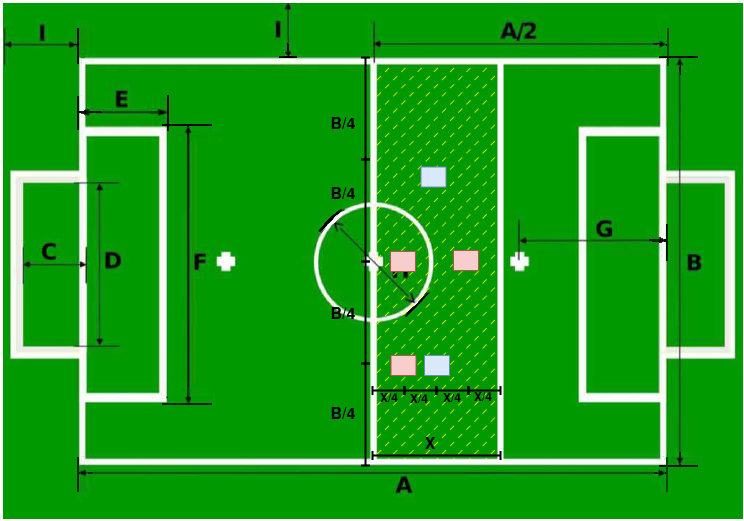
\includegraphics[width=\linewidth]{img/tcnavigation.png}
\caption{Setup for the Obstacle Navigation Challenge}
\label{fig:obs-nav}
\end{figure}

The goal of the Obstacle Navigation Challenge is demonstrate robots' ability to avoid collision with obstacles.

\vspace{2em}
{\bfseries Setup}

Figure~\ref{fig:obs-nav} shows the setup of the challenge.

A section of the field (marked dashed in yellow) is partitioned of using white tape.

The width of the field strip $X$ is 1.5m for KidSize and 3m for AdultSize. The length of the field strip $B$ is defined by the field sizes of KidSize and AdultSize.

Five obstacles are placed on the field. The obstacles are blue or red as specified by the team colors. Their height is 0.4m for KidSize and 1m for AdultSize. Their width is 0.4m for KidSize and 0.6m for AdultSize.

Nine locations are possible for obstacle placement at increments of $\frac{1}{4}$ X and B respectively. Not more than two obstacles shall be placed next to each other (i.e. at the same $\frac{1}{4}$ increment of B) to allow the robot to pass. The placement and color of obstacles shall be randomized for each attempt using for example the roll of a dice and/or a coin flip. \added{The placement of the outer obstacles (i.e. $\frac{1}{4}$ X and $\frac{3}{4}$ X) shall be adjusted so that the distance between the obstacles and the white tape is smaller than the width of the robot.}

\vspace{2em}
{\bfseries Execution}
\begin{enumerate}
\item The robot is placed on the side line of the field (marked as A in Figure~\ref{fig:obs-nav}) in the middle of the field strip.
\item Teams may start the robot manually by pressing a button.
\item A chronometer is started when the robot starts moving (including head movements).
\item The run stops when the robot fully exits the field strip or reaches the opposite side. The team may abort the run.
\item The chronometer is stopped when the robot touches the sideline on the opposite side of the field.

\end{enumerate}
\vspace{2em}
{\bfseries Evaluation}
\begin{itemize}
\item Failure
\begin{itemize}
\item The robot fully exits the field strip
\item The robot knocks over an obstacle
\end{itemize}
\item Partial success
\begin{itemize}
\item The robot partially exits the field strip or touches an obstacle but touches the sideline on the opposite side of the field.
\end{itemize}
\item Success
\begin{itemize}
\item The robot touches the sideline on the opposite side of the field and does not touch any obstacles and does not partially or fully exit the field strip.
\end{itemize}
\end{itemize}



\vspace{2em}
{\bfseries Ranking}

Teams are ranked on their best run according to the following criteria:
\begin{enumerate}
\item Duration of a \textit{Successful} run
\item Duration of a \textit{Partially Successful} run
\end{enumerate}